% History
% 12/06/2024  (岸)	修論下書き用texファイル作成
% 12/12/2024  (岸)	フォントサイズを11pt, 行間を1.5に設定
% コンパイルの仕方
% 		uplatex chapter1_v1.tex
% 		upbibtex chapter1_v1
% 		uplatex chapter1_v1.tex
% 		uplatex chapter1_v1.tex
% 		dvipdfmx chapter1_v1.dvi

% フォントサイズを11ptに設定
\documentclass[a4paper,11pt,nomag]{jsreport}

\usepackage[dvipdfm,truedimen]{geometry}
\geometry{top=22mm,bottom=22mm,left=22mm,right=22mm}
%% jsclasses系で文字サイズ11pt や 12pt をクラスオプションに指定すると,
%% 長さが拡大されるため,nomagオプションを併用している.
%% https://oku.edu.mie-u.ac.jp/~okumura/jsclasses/ のFAQをよく読むこと.

%\usepackage{layout}
%\usepackage[utf8]{inputenc} %不要かも
\usepackage[T1]{fontenc} %utf8フォントエンコーディング指定
\usepackage{lmodern} % 11pt, nomag を使っているので
% CloudLaTeX の場合は下の1行を有効にすること
% \AtBeginDvi{\special{pdf:mapfile ptex-ipaex.map}}
\usepackage{array}
\newcommand{\bhline}[1]{\noalign{\hrule height #1}}  
\newcommand{\bvline}[1]{\vrule width #1}
\renewcommand{\baselinestretch}{1.5} % 教授が赤修正を入れやすいように行間を1.5に設定
\usepackage[subrefformat=parens]{subcaption}
\usepackage[dvipdfmx]{graphicx} % dvipdfmx を前提としている
\usepackage[dvipdfmx]{color}
\usepackage{caption}
\usepackage{subcaption}
\usepackage{bbm}
\usepackage{multirow}
\usepackage{arydshln}
\usepackage{here} % 図表の位置決め用
\usepackage{amsmath,amssymb}% 数式用
\usepackage{url}      % URL等記載用.\verbより便利
\usepackage{enumerate}
\usepackage{midpage}

% サブキャプションのフォーマットを調整
\renewcommand\thesubfigure{(\alph{subfigure})}
\captionsetup[subfigure]{labelformat=simple, labelsep=space}

\begin{document}
\setcounter{chapter}{2}

\chapter*{深層学習を用いた動物分類に関する既存研究}

\section{赤外線画像に対する既存研究}

気候変動や人口増加が生態系に与える影響を把握し、野生動物と人間の持続可能な共存を実現することは、重要な課題である
この課題を解決するため、生態系モニタリングの重要性が世界的に高まっている\cite{zwerts2021, bandaru2024}。
生態系モニタリングの手法として、監視カメラなどを用いた観測が広く採用されており、特定地域における動物種の個体数推定だけでなく、環境に対する各動物種の生態の観察や研究が行われている\cite{trolliet2014}。
中でも、カメラトラップは、観察者による直接的な介入を最小限に抑えることが可能であり、観察者の存在が個体の行動に与える影響を軽減することができるため、野生動物の監視ツールとして広く活用されている\cite{本郷2018, abood2023}.
カメラトラップは,赤外線センサなどを用いた自動撮影により人的労力を削減することができ、近年のデジタルカメラの高性能化に伴い長期間にわたる連続的なモニタリングが可能である.
一方で、カメラトラップを使用した生態系モニタリングでは複数箇所にカメラトラップを設置するため、膨大な画像枚数を取得することも多く \cite{kays2020, si2014},記録された画像・動画中から人手による動物の有無や種の推定は多大なアノテーションコストを要する\cite{thangaraj2023}.
加えて,種の分類には専門的な知識が必要であることも作業員確保によるコスト面での課題である.
さらに、技術革新は今後も進むと予想されるのに対して、アノテーションコストを著しく下げることは困難であるため、このギャップは今後一層拡大していくと予想される\cite{安藤2019}。
したがって,これらの課題を解決するため,カメラトラップによって撮影された画像・動画中から自動で動物を検出・識別する手法の実現が望まれている.

近年では,画像処理技術と機械学習を用いた野生動物の自動識別手法が研究されている.
2012年の画像処理タスクに関連する深層学習技術の登場以降,画像処理分野の様々な分野においてCNNに基づく手法が盛んに研究されている.
また,その多くの分野においてCNNは高い性能を実現しており,カメラトラップによる動物識別に関する研究においてもCNNを用いた手法がいくつか提案されている.
Tanら \cite{tan2022}は,2014年から2020年にかけて撮影された約25,000枚の自作データセットを用いて,YOLOv5,FCOS(Fully Convolutional One-Stage ObjectDetection),Cascade R-CNNの3つの検出ネットワークでの比較検証をおよび映像に適用した動物認識の性能を評価している.
Tabakら \cite{tabak2019}は,全米5箇所で撮影された約300万枚のカメラトラップ画像を用いて,独自のCNNにより動物の画像分類を行っている.

しかしながら,上記のような既存研究の分類モデルを学習するために用いられた大規模なデータセットは,多くの撮影場所や数年間に及ぶ長期間の撮影によって蓄積された画像で構成されている.
したがって,これらの既存研究は,個人的な利用での撮影や狭い範囲の地域での撮影など,多くの画像を集められるとは限らない状況を考慮していないため実用的では無い.
また,夜間に行動する動物の撮影には赤外線カメラを用いることが有効である.
しかし,赤外線カメラで撮影された画像は色情報を含まないなど,可視光カメラで撮影された画像とは映り方が異なる.
したがって,真に実用的な夜間の動物モニタリングの実現に向けて,赤外線カメラを用いて撮影された少数の画像のみでも学習可能な深層学習モデルについての検討が急務である.

このような既存研究の課題解決に向けた研究として,少数の赤外線画像を用いた動物分類が挙げられる.
Kishiら \cite{kishimoto2023}は,米国南西部の140箇所で撮影された画像3,000枚を用いて,CNNによる少数の赤外線画像を用いた動物分類を行っている.
先行研究では,少数データを用いた効率的な深層学習モデルの学習を目的とするFSLの分野において有効な手法である転移学習とデータ拡張の赤外線画像に対する有効性が検証された.
転移学習は,事前に大量のデータを用いて学習したモデルを新しいタスクに適用する手法であり,先行研究では,画像認識タスクで一般的に用いられるImageNetデータセットとImageNetデータセットを擬似赤外線化した画像,さらに数式から生成されたフラクタル画像による転移学習の有効性が検証された.
一方,データ拡張については,一般的な画像変換に加え、画像の一部をマスクし隠すことでモデルの汎化性能を向上させるRandom Erasingや,複数の画像処理を組み合わせることで新しい画像を生成しモデルの頑健性を向上させるAugmixなどの有効性が検証された.
実験の結果,転移学習では疑似赤外線画像,フラクタル画像,ImageNetの順に効果が高いことが示され,データ拡張については,最新の手法であるAugMixが特に有効であることが明らかになった.

しかし,Kishiらの研究では,新規地域に対する深層学習モデルの適用開始時を想定しており,学習に使用する画像は1クラスあたり50枚としているが,実運用を想定すると1クラスあたり50枚程度の画像収集すら困難な場合も考えられる.
また,評価実験における評価用データセットでは学習用データセットと同じ動物種のみが使用されており,モデルの適用地域に生息する全ての動物種がモデルに登録されている閉集合が仮定されている.
モデルの実運用開始時において、対象地域に生息する全ての動物種のデータを網羅的に収集することは現実的ではない。
従来の分類モデルでは、学習データに含まれないモデルに未登録の動物を正しく識別できず、登録済みのクラスに強制的に分類されてしまうオープンセット問題が存在する。
% 特に重要な課題として,モデルの学習に使用されるデータに含まれる動物種が少ない場合,実用時には学習データに含まれなかった動物が出現することが挙げられる.
% 一般的な分類モデルは,そういった未見の動物を正しく識別できず,学習済みのクラスに強制的に分類してしまう.
図 \ref{fig:non_osr}は,従来の分類モデルが未登録の動物を識別できない例を示している.

\begin{figure}[tbp]
  \centering
  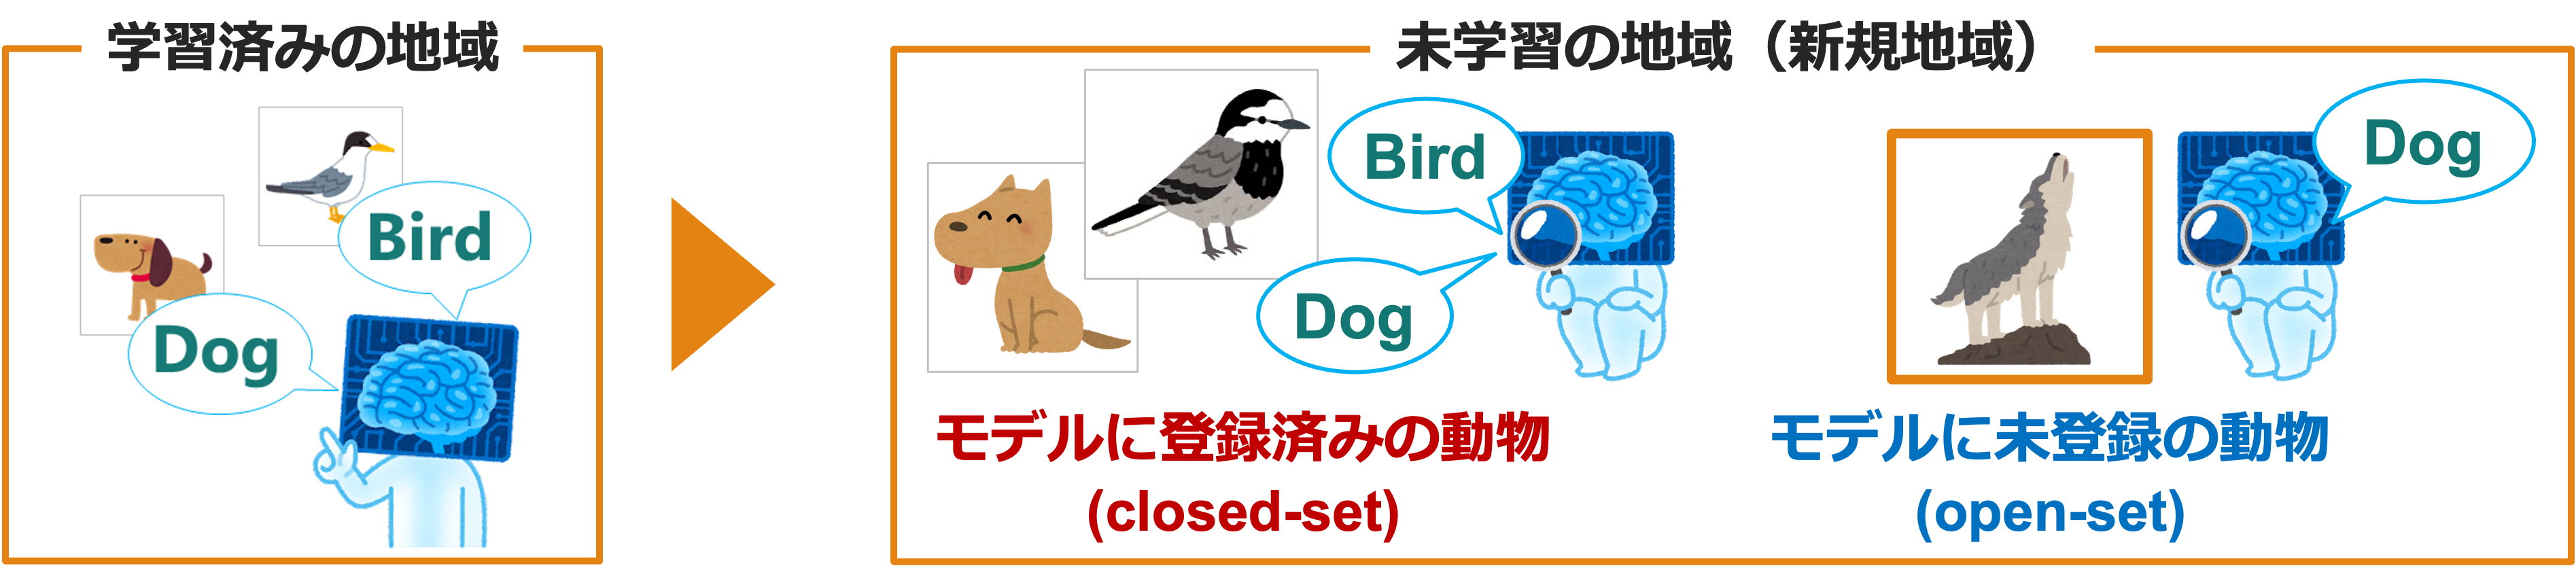
\includegraphics[width=\linewidth, keepaspectratio]{image/non_osr.png}
  \caption{従来の分類モデルによるオープンセット問題の例}
  \label{fig:non_osr}
\end{figure}

図\ref{fig:non_osr} に示される通り,犬と鳥のみを学習したモデルを新規地域に適用した場合、モデルに登録済みの犬や鳥は分類できるが、未登録の動物であるオオカミは登録済みの動物種に強制的に分類されてしまう。
このような誤分類はモデルの精度低下へと繋がるため、未登録の動物種を適切に検出できるOSRモデルの開発が急務となっている.
% 犬と一般的な分類モデルは分類したい画像を,画像から抽出した特徴量が類似している既存クラスに分類するため,未見データであっても等しく既存クラスに分類されてしまう.
% そのため,もし学習時データに含まれない危険な動物が実用時に現れた場合,モデルは判別することができず,重大な事故を引き起こす可能性がある.
以降、モデルに登録されている動物種セットをクローズドセット(closed-set)、モデルに未登録の動物種セットをオープンセット(open-set)と呼ぶ。


\subsection{Few-Shot Open-Set Recognitionに関する既存研究}




% ここから参考文献bibtexの設定
\bibliographystyle{../kishiIEEEtr}
\bibliography{../references}

\end{document}